\section{Auswertung}
\label{sec:Auswertung}

Im folgenden werden alle Meßunsicherheiten die aus Formeln mit fehlerbehafteten Größen stammen
mit der Gaußschen Fehlerfortpflanzung (Gl. \ref{eqn:Gauss}) berechnet.
\begin{equation}
    \Delta f =  \sqrt{\sum_{i=0}^n \left( \frac{\delta f}{\delta x_i} \cdot \Delta x_i\right)}   
    \label{eqn:Gauss}
\end{equation}

\subsection{Vorbereitung}
Als Vorbereitung werden die Energien $E_{\text{K}\alpha}$ und $E_{\text{K}\beta}$ für Kupfer recherchiert.
\begin{align*}
    E_{\text{K}\alpha} &= 8,038\text{keV}    &&   E_{\text{K}\beta} = 8,905\text{keV} \label{eqn:EnergieKupfer}
\end{align*}
Und es werden mit Gleichung \ref{eqn:Photon_Energie} die entsprechenden Wellenlängen für die Energien berechnet.
\begin{align*}
    E &= \frac{h\cdot c}{\lambda} && \lambda = \frac{h\cdot c}{E} \\
    \lambda_{\text{K}\alpha} &= 1,542\cdot 10^{-10} \text{m} \\
    \lambda_{\text{K}\beta} &= 1,392 \cdot 10^{-10} \text{m} 
\end{align*}
Über den Sinus werden aus den Wellenlängen die entsprechenden Glanzwinkel für die Brechungsordnung $n=1$ und einem LiF-Kristall mit $d = 201,4\cdot10^{-12} \text{m}$ berechnet.
\begin{align*}
   2d\sin{\alpha} &= n\lambda && \alpha = \arcsin \left(\frac{n\lambda}{2d}\right) \\
   \alpha_{\text{K}\alpha} &= 22.51° \\
   \alpha_{\text{K}\beta} &= 20.22°
\end{align*}
Außerdem wird als Referenz die Comptonwellenlänge des Elektrons theoretisch berechnet.
\begin{equation*}
    \lambda_{\text{C}} = \frac{h}{m_e c} = 2,42631 \cdot 10^{-12} \text{m}
\end{equation*}

\subsection{Kupfer Röntgenspektrum}
Aus den Kupfer Messwerten bildet sich:
\begin{figure}[H]
    \centering
    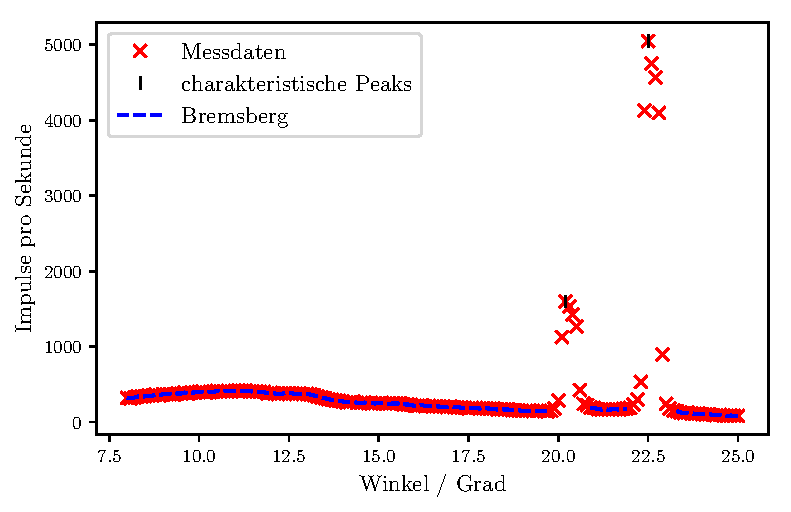
\includegraphics[width=0.7\textwidth]{plots/CU_Spektrum.pdf}
    \caption{Kupfer Emissionsspektrum mit Peaks und Bremsberg}
    \label{fig:CU_Spektrum}
\end{figure}
Mit einer Scipy Funktion werden die Peaks bei 1599 Impulsen pro Sekunde bei 20,2° und 5050 Impulsen pro Sekunde bei 22,5° gefunden.
Über die abgelesenen Winkel an den Peaks lassen sich nun die entsprechenden Energien berechnen(Gl. \ref{eqn:Bragg_Gleichung}).
\begin{align*}
    \alpha_{K\alpha} &= 22,5° &&   \alpha_{K\beta} = 20,2° \\
    E &= \frac{hc}{2d\sin(\alpha)} \\
    E_{K\alpha} &= 8043 \; eV && E_{K\beta} = 8914\; eV \label{eqn:Energien_Spektrum}
\end{align*}

\subsection{Wellenlängenabhängigkeit der Transmission}
Mit der Totzeitkorrektur (Gl. \ref{eqn:Totzeitkorrektur}) lässt sich aus den Impulsraten die korrigierte Rate berechnen.
Aus der berechneten Rate kann mit Gleichung \ref{eqn:Transmission} die Transmission für die entsprechende Wellenlänge gemessen werden.
Die Transmission wird gegen die Wellenlänge aufgetragen und mit einer linearen Ausgleichsrechnung die Funktion $T(\lambda)$ bestimmt.
\begin{equation}
    T = \frac{I_{\text{A}}}{I_0} \label{eqn:Transmission}
\end{equation}
\begin{figure}[H]
    \centering
    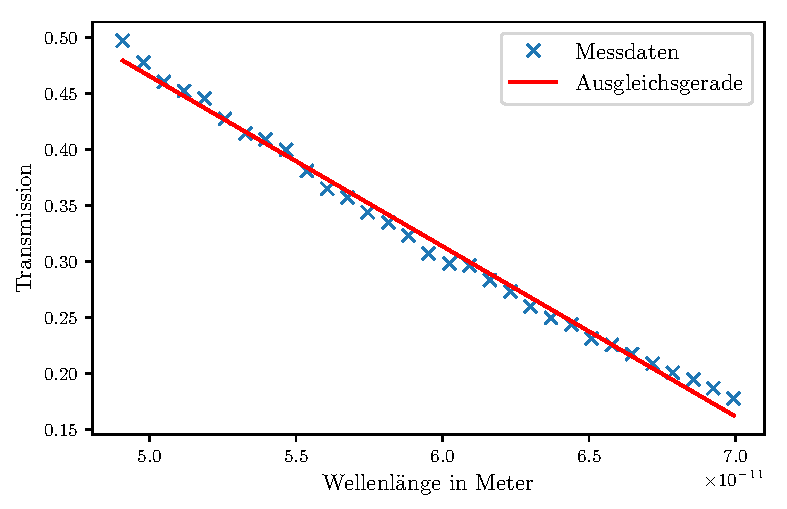
\includegraphics[width=0.7\textwidth]{plots/Transmission.pdf}
    \caption{Transmission von LiF in Abhängigkeit von der Wellenlänge}
    \label{fig:Transmission}
\end{figure}
Mit den Parametern und den Unsicherheiten aus der Covarianzmatrix ergibt sich:
\begin{align*}
    T(\lambda) = m \cdot \lambda + b  \\
    m = -0,0152 \pm 0,0003 \frac{1}{m}&& b= 1,23 \pm 0,02 
\end{align*}

\subsection{Comptonwellenlänge}
Im folgenden wird nun über die Transmission die Compton-Wellenlänge bestimmt.
Dafür werden die Impulsraten von den gestreuten und ungestreuten Photonen mit Gleichung \ref{eqn:Transmission} in die entsprechende Transmission umgerechnet.
\begin{align*}
    I_{\text{gestreut}} &= 1180 \pm 34  \\ 
    I_{\text{ungestreut}} &= 1024 \pm 32  \\
    I_0 &= 2730 \pm 50 \\
    T_1 &= 0,0432 \pm 0,015 \\
    T_2 &= 0,375 \pm 0,014 \\ 
\end{align*}
\begin{align*}
    \lambda &= \frac{T-b}{m} \\
    \lambda_{1} &=  (52,2 \pm 1,6) \cdot 10^{-12} \text{m}\\
    \lambda_{2} &=  (55,9 \pm 1,6) \cdot 10^{-12} \text{m}
\end{align*}
Über Gleichung \ref{eqn:Compton_Gesetz} lässt sich über die Wellenlängendifferenz die Comptonwellenlänge des Elektrons bestimmen.
Die Differenz der Wellenlängen entspricht der Comptonwellenlänge da die Strahlung genau im 90° Winkel gestreut wird.
\begin{equation*}
    \Delta\lambda = \lambda_{\text{C}} = (3,8\pm 1,1)\cdot 10^{-12} \text{m}
\end{equation*}

